% answers.tex —— 1997 年·上海卷·文史类 · 参考答案与详细解析片段
% 由 tools/generate_projects.py 依来源总账自 1997/1997_数学真题_上海文_试题.md + 1997/1997_数学真题_上海文_解析正文.md + 1997/1997_数学真题_上海文_答案要点.md 生成，勿手改（改源 MD 后重跑）


\begin{answer}
\gksolhead{1}{}

\textbf{题目}：

设全集是实数集 $\mathbb R$，$M=\{x\mid x\le 1+\sqrt2,\ x\in\mathbb R\}$，$N=\{1,2,3,4\}$，则 $\overline M\cap N$ 等于\mbox{（　　）}

（A）$\{4\}$　（B）$\{3,4\}$　（C）$\{2,3,4\}$　（D）$\{1,2,3,4\}$

\Needspace{4\baselineskip}
\textbf{解析}

本题为选择题，固定来源仅印载答案，未印推导；答案见「答案要点」，此处不补写来源未载的解析。

\gkanswer{答案：B。}

\end{answer}
\begin{answer}
\gksolhead{2}{}

\textbf{题目}：

三个数 $6^{0.7}$、$0.7^6$、$\log_{0.7}6$ 的大小顺序是\mbox{（　　）}

（A）$0.7^6<\log_{0.7}6<6^{0.7}$　（B）$0.7^6<6^{0.7}<\log_{0.7}6$

（C）$\log_{0.7}6<6^{0.7}<0.7^6$　（D）$\log_{0.7}6<0.7^6<6^{0.7}$

\Needspace{4\baselineskip}
\textbf{解析}

本题为选择题，固定来源仅印载答案，未印推导；答案见「答案要点」，此处不补写来源未载的解析。

\gkanswer{答案：D。}

\end{answer}
\begin{answer}
\gksolhead{3}{}

\textbf{题目}：

在下列命题中，假命题是\mbox{（　　）}

（A）若 $a,b$ 是异面直线，则一定存在平面 $\alpha$ 过 $a$ 且与 $b$ 平行。

（B）若 $a,b$ 是异面直线，则一定存在平面 $\alpha$ 过 $a$ 且与 $b$ 垂直。

（C）若 $a,b$ 是异面直线，则一定存在平面 $\alpha$，与 $a,b$ 所成角相等。

（D）若 $a,b$ 是异面直线，则一定存在平面 $\alpha$，与 $a,b$ 的距离相等。

\Needspace{4\baselineskip}
\textbf{解析}

本题为选择题，固定来源仅印载答案，未印推导；答案见「答案要点」，此处不补写来源未载的解析。

\gkanswer{答案：B。}

\end{answer}
\begin{answer}
\gksolhead{4}{}

\textbf{题目}：

设 $k>1$，则关于 $x,y$ 的方程 $(1-k)x^2+y^2=k^2-1$ 所表示的曲线是\mbox{（　　）}

（A）长轴在 $y$ 轴上的椭圆　（B）长轴在 $x$ 轴上的椭圆

（C）实轴在 $y$ 轴上的双曲线　（D）实轴在 $x$ 轴上的双曲线

\Needspace{4\baselineskip}
\textbf{解析}

本题为选择题，固定来源仅印载答案，未印推导；答案见「答案要点」，此处不补写来源未载的解析。

\gkanswer{答案：C。}

\end{answer}
\begin{answer}
\gksolhead{5}{}

\textbf{题目}：

如果直线 $l$ 沿 $x$ 轴负方向平移 3 个单位，再沿 $y$ 轴正方向平移 1 个单位后，又回到原来的位置，那么直线 $l$ 的斜率是\mbox{（　　）}

（A）$-\dfrac13$　（B）$-3$　（C）$\dfrac13$　（D）$3$

\Needspace{4\baselineskip}
\textbf{解析}

本题为选择题，固定来源仅印载答案，未印推导；答案见「答案要点」，此处不补写来源未载的解析。

\gkanswer{答案：A。}

\end{answer}
\begin{answer}
\gksolhead{6}{}

\textbf{题目}：

设 $f(n)=1+\dfrac12+\dfrac13+\cdots+\dfrac1{3n-1}$（$n\in\mathbb N$），则 $f(n+1)-f(n)$ 等于\mbox{（　　）}

（A）$\dfrac1{3n+2}$　（B）$\dfrac1{3n}+\dfrac1{3n+1}$

（C）$\dfrac1{3n+1}+\dfrac1{3n+2}$　（D）$\dfrac1{3n}+\dfrac1{3n+1}+\dfrac1{3n+2}$

\Needspace{4\baselineskip}
\textbf{解析}

本题为选择题，固定来源仅印载答案，未印推导；答案见「答案要点」，此处不补写来源未载的解析。

\gkanswer{答案：D。}

\end{answer}
\begin{answer}
\gksolhead{7}{}

\textbf{题目}：

方程 $\lg(1-3x)=\lg(3-x)+\lg(7+x)$ 的解是 \gkblank{}。

\Needspace{4\baselineskip}
\textbf{解析}

本题为填空题，固定来源仅印载答案，未印推导；答案见「答案要点」，此处不补写来源未载的解析。

\gkanswer{答案：$x=-5$。}

\end{answer}
\begin{answer}
\gksolhead{8}{}

\textbf{题目}：

方程 $\sin 2x=\dfrac12$ 在区间 $[-2\pi,2\pi]$ 内解的个数是 \gkblank{}。

\Needspace{4\baselineskip}
\textbf{解析}

本题为填空题，固定来源仅印载答案，未印推导；答案见「答案要点」，此处不补写来源未载的解析。

\gkanswer{答案：$8$。}

\end{answer}
\begin{answer}
\gksolhead{9}{}

\textbf{题目}：

已知 $a=\dfrac{-3-i}{1+2i}$（$i$ 是虚数单位），那么 $a^2=$ \gkblank{}。

\Needspace{4\baselineskip}
\textbf{解析}

本题为填空题，固定来源仅印载答案，未印推导；答案见「答案要点」，此处不补写来源未载的解析。

\gkanswer{答案：$-2i$。}

\end{answer}
\begin{answer}
\gksolhead{10}{}

\textbf{题目}：

设圆 $x^2+y^2-4x-5=0$ 的弦 $AB$ 的中点为 $P(3,1)$，则直线 $AB$ 的方程是 \gkblank{}。

\Needspace{4\baselineskip}
\textbf{解析}

本题为填空题，固定来源仅印载答案，未印推导；答案见「答案要点」，此处不补写来源未载的解析。

\gkanswer{答案：$x+y-4=0$。}

\end{answer}
\begin{answer}
\gksolhead{11}{}

\textbf{题目}：

若 $(3x+1)^n$（$n\in\mathbb N$）的展开式中各项系数的和是 256，则展开式中 $x^2$ 的系数是 \gkblank{}。

\Needspace{4\baselineskip}
\textbf{解析}

本题为填空题，固定来源仅印载答案，未印推导；答案见「答案要点」，此处不补写来源未载的解析。

\gkanswer{答案：$54$。}

\end{answer}
\begin{answer}
\gksolhead{12}{}

\textbf{题目}：

函数 $f(x)=3\sin x\cos x-1$ 的最大值是 \gkblank{}。

\Needspace{4\baselineskip}
\textbf{解析}

本题为填空题，固定来源仅印载答案，未印推导；答案见「答案要点」，此处不补写来源未载的解析。

\gkanswer{答案：$\dfrac12$。}

\end{answer}
\begin{answer}
\gksolhead{13}{}

\textbf{题目}：

$A_1$组（非试点校）：设 $0<a<b$，则 $\displaystyle\lim_{n\to\infty}\frac{4b^n}{a^n-b^n}=$ \gkblank{}。

$B_1$组（试点校）：$\displaystyle\lim_{n\to\infty}\left(1-\frac2n\right)^{-2n}=$ \gkblank{}。

\Needspace{4\baselineskip}
\textbf{解析}

本题为填空题，固定来源仅印载答案，未印推导（$A_1$/$B_1$ 两组答案见答案要点）；答案见「答案要点」，此处不补写来源未载的解析。

\gkanswer{答案：$A_1$ 组 $-4$；$B_1$ 组 $e^4$。}

\end{answer}
\begin{answer}
\gksolhead{14}{}

\textbf{题目}：

$A_1$组（非试点校）：设正四棱锥底面边长为 $4\,\mathrm{cm}$，侧面和底面所成的二面角是 $60^\circ$，则这个棱锥的侧面积是 \gkblank{} $\mathrm{cm}^2$。

$B_1$组（试点校）：设 $\vec a=(m+1)\vec i-3\vec j$，$\vec b=\vec i+(m-1)\vec j$，$(\vec a+\vec b)\perp(\vec a-\vec b)$，则 $m=$\gkblank{}。

\Needspace{4\baselineskip}
\textbf{解析}

本题为填空题，固定来源仅印载答案，未印推导（$A_1$/$B_1$ 两组答案见答案要点）；答案见「答案要点」，此处不补写来源未载的解析。

\gkanswer{答案：$A_1$ 组 $32\,\mathrm{cm}^2$；$B_1$ 组 $-2$。}

\end{answer}
\begin{answer}
\gksolhead{15}{}

\textbf{题目}：

$A_1$组（非试点校）：圆柱形容器的内壁底半径为 $5\,\mathrm{cm}$，两个直径为 $5\,\mathrm{cm}$ 的玻璃小球都浸没于容器的水中。若取出这两个小球，则容器内的水面将下降 \gkblank{} $\mathrm{cm}$。

$B_1$组（试点校）：设 $f(x)=x^2(2-x)$，则 $f(x)$ 的单调递增区间是 \gkblank{}。

\Needspace{4\baselineskip}
\textbf{解析}

本题为填空题，固定来源仅印载答案，未印推导（$A_1$/$B_1$ 两组答案见答案要点）；答案见「答案要点」，此处不补写来源未载的解析。

\gkanswer{答案：$A_1$ 组 $\dfrac53\,\mathrm{cm}$；$B_1$ 组 $\left(0,\dfrac43\right)$。}

\end{answer}
\begin{answer}
\gksolhead{16}{}

\textbf{题目}：

$A_1$组（非试点校）：从集合 $\{0,1,2,3,5,7,11\}$ 中任取 3 个元素分别作为直线方程 $Ax+By+C=0$ 中的 $A,B,C$，所得经过坐标原点的直线有 \gkblank{} 条（结果用数值表示）。

$B_1$组（试点校）：从集合 $\{0,1,2,3,5,7,11\}$ 中任取 3 个元素分别作为直线方程 $Ax+By+C=0$ 中的 $A,B,C$，所得恰好经过坐标原点的直线的概率是 \gkblank{}。

\Needspace{4\baselineskip}
\textbf{解析}

本题为填空题，固定来源仅印载答案，未印推导（$A_1$/$B_1$ 两组答案见答案要点）；答案见「答案要点」，此处不补写来源未载的解析。

以下按固定来源 PDF“数学试卷答案及评分标准”转录第 17—22 题中印载的解答步骤；使用统一 LaTeX 记号整理排版，不把来源内容表述为已核实的官方答案或独立验证。来源题面、解析与评分均待另一审阅者逐页核对。

\gkanswer{答案：$A_1$ 组 $30$；$B_1$ 组 $\dfrac17$。}

\end{answer}
\begin{answer}
\gksolhead{17}{}

\textbf{题目}（10分）：

已知 $\tan\dfrac\alpha2=\dfrac12$，求 $\sin\left(\alpha+\dfrac\pi6\right)$ 的值。

\Needspace{4\baselineskip}
\textbf{解析}

\Needspace{5\baselineskip}
\textbf{解法一：}

\nopagebreak[4]
\[\sin\alpha=\frac{2\tan(\alpha/2)}{1+\tan^2(\alpha/2)}=\frac{2\times\frac12}{1+\frac14}=\frac45\quad(3\text{\text{分}}),\]
\nopagebreak[4]
\[\cos\alpha=\frac{1-\tan^2(\alpha/2)}{1+\tan^2(\alpha/2)}=\frac{1-\frac14}{1+\frac14}=\frac35\quad(6\text{\text{分}}).\]

\Needspace{5\baselineskip}
于是
\nopagebreak[4]
\[\sin\left(\alpha+\frac\pi6\right)=\sin\alpha\cos\frac\pi6+\cos\alpha\sin\frac\pi6
=\frac45\cdot\frac{\sqrt3}{2}+\frac35\cdot\frac12
=\frac{3+4\sqrt3}{10}\quad(10\text{\text{分}}).\]

\Needspace{5\baselineskip}
\textbf{解法二：} 来源解答由 $\tan(\alpha/2)=1/2$ 判断 $\alpha$ 为第一象限角，再用
\nopagebreak[4]
\[\tan\alpha=\frac{2\tan(\alpha/2)}{1-\tan^2(\alpha/2)}=\frac43,\]
得到 $\cos\alpha=3/5,\ \sin\alpha=4/5$，代入和角公式，结论相同。

\gkanswer{答案：$\sin\left(\alpha+\dfrac\pi6\right)=\dfrac{3+4\sqrt3}{10}$。}

\end{answer}
\begin{answer}
\gksolhead{18}{}

\textbf{题目}（10分）：

公园要建造一个圆形的喷水池。在水池中央垂直于水面安装一个花形柱子 $OA$，$O$ 恰在水面中心，$OA=1.25$ 米。安置在柱子顶端 $A$ 处的喷头向外喷水，水流在各个方向上沿形状相同的抛物线路径落下，且在过 $OA$ 的任一平面上抛物线路径如图所示。为使水流形状较为漂亮，设计成水流在到 $OA$ 距离为 1 米处达到距水面最大高度 2.25 米。如果不计其他因素，那么水池的半径至少要多少米，才能使喷出的水流不致落到池外？
\nopagebreak[4]
\begin{center}% 依据固定来源示意图重绘；曲线依据题干数据示意，不按比例。
\begin{tikzpicture}[x=0.85cm,y=0.65cm,line cap=round,line join=round]
  \draw[thick] (-3.1,0)--(3.1,0) node[right]{水面};
  \draw[thick] (0,0)--(0,1.25);
  \fill (0,1.25) circle (1.4pt) node[left]{A};
  \fill (0,0) circle (1.4pt) node[below left]{O};
  \draw[thick,domain=0:2.5,samples=80] plot (\x,{-(\x-1)^2+2.25});
  \draw[thick,domain=-2.5:0,samples=80] plot (\x,{-(\x+1)^2+2.25});
\end{tikzpicture}
\end{center}
\nopagebreak[4]
\Needspace{4\baselineskip}
\textbf{解析}

\Needspace{5\baselineskip}
如图建立直角坐标系，设水流轨迹为
\nopagebreak[4]
\[y=a(x-1)^2+2.25.\]
\Needspace{5\baselineskip}
由题意，点 $A$ 的坐标为 $(0,1.25)$。把 $x=0$、$y=1.25$ 代入，得 $a=-1$，所以
\nopagebreak[4]
\[y=-(x-1)^2+2.25.\]
令 $y=0$，得 $-(x-1)^2+2.25=0$，解得 $x_1=2.5$、$x_2=-0.5$；负根不合题意，舍去。故水池半径至少为 $2.5$ 米，才能使水流不落到池外。

\gkanswer{答案：水池半径至少 $2.5$ 米。}

\end{answer}
\begin{answer}
\gksolhead{19}{}

\textbf{题目}（14分）：

本题共有 2 个小题，第 1 小题满分 6 分，第 2 小题满分 8 分。如图，在三棱柱 $ABC-A'B'C'$ 中，四边形 $A'ABB'$ 是菱形，四边形 $BCC'B'$ 是矩形，$C'B'\perp AB$。

（1）求证：平面 $CA'B\perp$ 平面 $A'AB$；

（2）若 $C'B'=3$，$AB=4$，$\angle ABB'=60^\circ$，求 $AC'$ 与平面 $BCC'$ 所成角的大小（用反三角函数表示）。
\nopagebreak[4]
\begin{center}% 三棱柱拓扑示意；投影不按比例，虚线表示遮挡的棱/辅助连线。
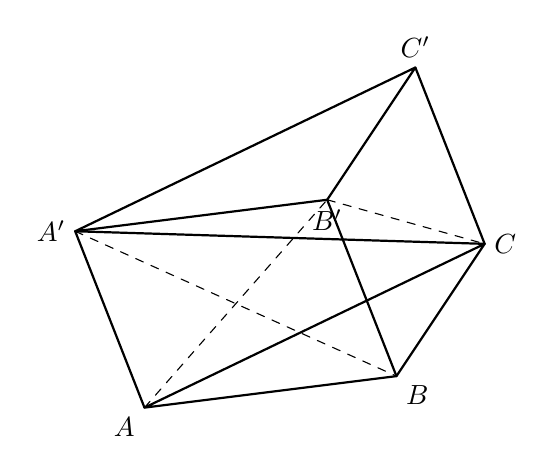
\begin{tikzpicture}[x=0.8cm,y=0.8cm,line cap=round,line join=round]
  \coordinate (A)  at (0,0);
  \coordinate (B)  at (4,0.5);
  \coordinate (C)  at (5.4,2.6);
  \coordinate (Ap) at (-1.1,2.8);
  \coordinate (Bp) at (2.9,3.3);
  \coordinate (Cp) at (4.3,5.4);
  \draw[thick] (A)--(B)--(C)--cycle;
  \draw[thick] (Ap)--(Bp)--(Cp)--cycle;
  \draw[thick] (A)--(Ap) (B)--(Bp) (C)--(Cp);
  \draw[thick] (Ap)--(C);
  \draw[dashed] (Ap)--(B) (A)--(Bp) (Bp)--(C);
  \node[below left] at (A) {$A$};
  \node[below right] at (B) {$B$};
  \node[right] at (C) {$C$};
  \node[left] at (Ap) {$A'$};
  \node[below] at (Bp) {$B'$};
  \node[above] at (Cp) {$C'$};
\end{tikzpicture}
\end{center}
\nopagebreak[4]
\Needspace{4\baselineskip}
\textbf{解析}

（1）在三棱柱 $ABC-A'B'C'$ 中，$C'B'\parallel CB$。由 $C'B'\perp AB$，得 $CB\perp AB$；又 $CB\perp BB'$，且 $AB\cap BB'=B$，所以 $CB\perp$ 平面 $A'AB$。又 $CB\subset$ 平面 $CA'B$，因此平面 $CA'B\perp$ 平面 $A'AB$。（累计 3、6 分）

（2）由 $C'B'\perp$ 平面 $A'AB$，得平面 $A'AB\perp$ 平面 $BCC'$。过 $A$ 作 $AH\perp$ 平面 $BCC'$，垂足为 $H$，则 $H$ 在 $BB'$ 上。连接 $C'H$，则 $\angle AC'H$ 为直线 $AC'$ 与平面 $BCC'$ 所成的角。（10分）

\Needspace{5\baselineskip}
连接 $AB'$。由四边形 $A'ABB'$ 是菱形且 $\angle ABB'=60^\circ$，可知 $\triangle ABB'$ 为等边三角形，$H$ 为 $BB'$ 中点。又 $AB'=4$、$AH=2\sqrt3$，在直角三角形 $C'B'A$ 中有 $AC'=\sqrt{4^2+3^2}=5$；在直角三角形 $AHC'$ 中，
\nopagebreak[4]
\[\sin\angle AC'H=\frac{AH}{AC'}=\frac{2\sqrt3}{5}.\]
所以所求角为 $\arcsin\dfrac{2\sqrt3}{5}$。（14分）

\gkanswer{答案：（1）证明见解析；（2）$\arcsin\dfrac{2\sqrt3}{5}$。}

\end{answer}
\begin{answer}
\gksolhead{20}{}

\textbf{题目}（16分）：

$A_2$组（非试点校，本题共 2 小题，第 1 小题、第 2 小题各 8 分）：设虚数 $z_1,z_2$ 满足 $z_1^2=z_2$。

（1）若 $z_1,z_2$ 又是一个实系数一元二次方程的两个根，求 $z_1,z_2$；

（2）若 $z_1=1+mi$（$i$ 为虚数单位），$|z_1|\le\sqrt2$，复数 $\omega=z_2+3$，求 $|\omega|$ 的取值范围。

$B_2$组（试点校，本题第 1 小题 6 分、第 2 小题 10 分）：如图，抛物线 $C_1:y=-x^2$ 与抛物线 $C_2:y=x^2-2ax$（$a>0$）交于 $O,A$ 两点。

（1）把 $C_1$ 与 $C_2$ 所围成的图形（阴影部分）绕 $x$ 轴旋转一周，求所得几何体的体积 $V$；

（2）若过原点的直线 $l$ 与抛物线 $C_2$ 所围成的图形面积为 $\dfrac92a^3$，求直线 $l$ 的方程。
\nopagebreak[4]
\begin{center}% C1、C2 与阴影区域的示意重绘；图中取 a=1 仅为排布，非题设附加条件。
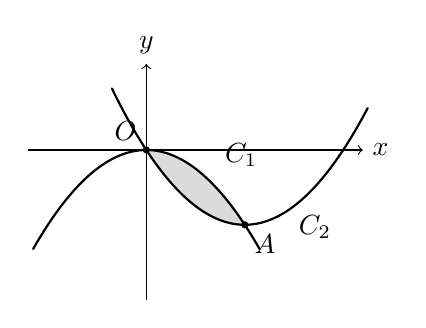
\begin{tikzpicture}[x=1.25cm,y=0.95cm,line cap=round,line join=round]
  \fill[gray!28] (0,0)
    -- plot[domain=0:1,samples=60] (\x,{-\x*\x})
    -- plot[domain=1:0,samples=60] (\x,{\x*\x-2*\x}) -- cycle;
  \draw[->] (-1.2,0)--(2.2,0) node[right] {$x$};
  \draw[->] (0,-2.0)--(0,1.15) node[above] {$y$};
  \draw[thick,domain=-1.15:1.15,samples=80] plot (\x,{-\x*\x});
  \draw[thick,domain=-0.35:2.25,samples=80] plot (\x,{\x*\x-2*\x});
  \fill (0,0) circle (1.3pt) node[above left] {$O$};
  \fill (1,-1) circle (1.3pt) node[below right] {$A$};
  \node[above right] at (0.7,-0.35) {$C_1$};
  \node[below right] at (1.45,-0.75) {$C_2$};
\end{tikzpicture}
\end{center}
\nopagebreak[4]
\Needspace{4\baselineskip}
\textbf{解析}

\gksubpart{$A_2$ 组（16 分）}
\Needspace{5\baselineskip}
（1）\textbf{解法一：} 设 $z_1=a+bi,\ z_2=a-bi$，其中 $a,b\in\mathbb R$ 且 $b\ne0$。由 $z_1^2=z_2$，
\nopagebreak[4]
\[a^2-b^2+2abi=a-bi,\]
\Needspace{5\baselineskip}
从而 $a^2-b^2=a$、$2ab=-b$。解得 $a=-1/2$、$b=\pm\sqrt3/2$。因此
\nopagebreak[4]
\[z_1=-\frac12+\frac{\sqrt3}{2}i,\quad z_2=-\frac12-\frac{\sqrt3}{2}i,\]
或两者互换。（累计 2、6、8 分）

\textbf{解法二：} 设实系数一元二次方程为 $z^2+pz+q=0$，且 $p^2-4q<0$。由求根公式写出共轭两根，再利用 $z_1^2=z_2$ 比较实部、虚部，解得 $p=q=1$，于是两根为 $-\dfrac12\pm\dfrac{\sqrt3}{2}i$，并按 $z_1^2=z_2$ 配对。（来源原页此解法给出相同的两种有序配对；累计 2、6、8 分）

\Needspace{5\baselineskip}
（2）由 $z_1=1+mi$、$|z_1|\le\sqrt2$ 且 $m\ne0$，得 $0<m^2\le1$。又 $z_2=z_1^2$、$\omega=z_2+3$，故
\nopagebreak[4]
\[\omega=(4-m^2)+2mi,\]
\nopagebreak[4]
\[|\omega|=\sqrt{(4-m^2)^2+4m^2}=\sqrt{(m^2-2)^2+12}.\]
\Needspace{5\baselineskip}
由 $0<m^2\le1$，得 $13\le(m^2-2)^2+12<16$，所以
\nopagebreak[4]
\[|\omega|\in[\sqrt{13},4).\]

\gksubpart{$B_2$ 组（16 分）}
\Needspace{5\baselineskip}
（1）$C_1$ 与 $C_2$ 交于 $O(0,0)$、$A(a,-a^2)$。绕 $x$ 轴旋转一周所得体积为
\nopagebreak[4]
\[\begin{aligned}
V&=\pi\int_0^a(x^2-2ax)^2\,dx-\pi\int_0^a(-x^2)^2\,dx\\
&=4a\pi\int_0^a(-x^3+ax^2)\,dx\\
&=4a\pi\left(-\frac14x^4+\frac13ax^3\right)_0^a
=\frac{\pi a^5}{3}.
\end{aligned}\]
（累计 2、6 分）

\Needspace{5\baselineskip}
（2）设过原点的直线为 $y=kx$。联立 $y=kx$ 与 $y=x^2-2ax$，交点横坐标为 $0$、$k+2a$。当 $k+2a\ge0$ 时，所围面积
\nopagebreak[4]
\[S=\int_0^{k+2a}\bigl(kx-x^2+2ax\bigr)\,dx=\frac{(k+2a)^3}{6}.\]
由 $S=\dfrac92a^3$ 得 $(k+2a)^3=27a^3$，故 $k=a$，直线为 $y=ax$。（累计 8、12 分）

\Needspace{5\baselineskip}
当 $k+2a<0$ 时，
\nopagebreak[4]
\[S=\int_{k+2a}^{0}\bigl((k+2a)x-x^2\bigr)\,dx=-\frac{(k+2a)^3}{6}.\]
由 $S=\dfrac92a^3$ 得 $-(k+2a)^3=27a^3$，故 $k=-5a$，直线为 $y=-5ax$。（16分）

\gkanswer{答案：$A_2$ 组（1）$(z_1,z_2)=\left(-\dfrac12+\dfrac{\sqrt3}{2}i,\ -\dfrac12-\dfrac{\sqrt3}{2}i\right)$ 或互换；（2）$|\omega|\in[\sqrt{13},4)$。$B_2$ 组（1）$V=\dfrac{\pi a^5}{3}$；（2）$y=ax$ 或 $y=-5ax$。}

\end{answer}
\begin{answer}
\gksolhead{21}{}

\textbf{题目}（18分）：

本题共有 3 个小题，第 1 小题满分 5 分，第 2 小题满分 6 分，第 3 小题满分 7 分。如图，抛物线方程为 $y^2=p(x+1)$（$p>0$），直线 $x+y=m$ 与 $x$ 轴的交点在抛物线的准线右边。

（1）求证：直线与抛物线总有两个交点；

（2）设直线与抛物线的交点为 $Q,R$，$OQ\perp OR$，求 $p$ 关于 $m$ 的函数 $p=f(m)$ 的表达式；

（3）在（2）的条件下，若抛物线焦点 $F$ 到直线 $x+y=m$ 的距离为 $\dfrac{\sqrt2}{2}$，求此直线的方程。
\nopagebreak[4]
\begin{center}% 抛物线、焦点、准线右侧截距与直线示意；本图取 p=1、m=0.1，仅示关系，不按比例。
\begin{tikzpicture}[x=1.05cm,y=1.05cm,line cap=round,line join=round]
  \draw[->] (-1.5,0)--(2.65,0) node[right] {$x$};
  \draw[->] (0,-2.15)--(0,1.45) node[above] {$y$};
  \draw[densely dashed] (-1.25,-1.9)--(-1.25,1.3) node[above] {准线};
  \draw[thick,domain=-1.8:1.2,samples=90] plot ({\x*\x-1},{\x});
  \draw[thick,domain=-1.9:1.2,samples=80] plot ({0.1-\x},{\x});
  \fill (0,0) circle (1.3pt) node[below right] {$O$};
  \fill (-0.75,0) circle (1.3pt) node[below] {$F$};
  \fill (-0.56,0.66) circle (1.3pt) node[above left] {$Q$};
  \fill (1.76,-1.66) circle (1.3pt) node[below right] {$R$};
\end{tikzpicture}
\end{center}
\nopagebreak[4]
\Needspace{4\baselineskip}
\textbf{解析}

（1）抛物线 $y^2=p(x+1)$ 的准线为 $x=-1-p/4$。直线 $x+y=m$ 与 $x$ 轴交于 $(m,0)$；交点在准线右边，所以 $m>-1-p/4$，即 $4m+p+4>0$。（累计 3分）

\Needspace{5\baselineskip}
联立
\nopagebreak[4]
\[\begin{cases}y^2=p(x+1),\\x+y=m,\end{cases}\]
\Needspace{5\baselineskip}
消去 $y$，得
\nopagebreak[4]
\[x^2-(2m+p)x+(m^2-p)=0.\]
\Needspace{5\baselineskip}
其判别式
\nopagebreak[4]
\[\Delta=(2m+p)^2-4(m^2-p)=p(4m+p+4)>0,\]
因此直线与抛物线总有两个交点。（5分）

\Needspace{5\baselineskip}
（2）设 $Q,R$ 的坐标分别为 $(x_1,y_1),(x_2,y_2)$。由上式，$x_1,x_2$ 是方程 $x^2-(2m+p)x+m^2-p=0$ 的两根，故 $x_1+x_2=2m+p$、$x_1x_2=m^2-p$。由 $OQ\perp OR$，有 $x_1x_2+y_1y_2=0$。又 $Q,R$ 在直线 $x+y=m$ 上，故 $y_1=m-x_1$、$y_2=m-x_2$。于是
\nopagebreak[4]
\[x_1x_2+y_1y_2=2x_1x_2-m(x_1+x_2)+m^2=0,\]
\Needspace{5\baselineskip}
代入根与系数的关系得 $p(m+2)=m^2$，所以
\nopagebreak[4]
\[p=f(m)=\frac{m^2}{m+2},\qquad m>-2,\ m\ne0.\]
（累计 7、11分）

\Needspace{5\baselineskip}
（3）抛物线焦点 $F$ 的坐标为 $(-1+p/4,0)$。由点到直线的距离条件，
\nopagebreak[4]
\[\frac{|p/4-1-m|}{\sqrt2}=\frac{\sqrt2}{2},\qquad |p-4m-4|=4.\]
\Needspace{5\baselineskip}
代入 $p=m^2/(m+2)$，得
\nopagebreak[4]
\[\left|\frac{3m^2+12m+8}{m+2}\right|=4.\]
\Needspace{5\baselineskip}
解得 $m_1=0,\ m_2=-8/3,\ m_3=-4,\ m_4=-4/3$。由 $m\ne0$ 且 $m>-2$，舍去前三个值，故直线方程为 $x+y=-4/3$，即
\nopagebreak[4]
\[3x+3y+4=0.\]
（累计 13、16、18分）

\gkanswer{答案：（1）证明见解析；（2）$p=\dfrac{m^2}{m+2}$（$m>-2$，$m\ne0$）；（3）$3x+3y+4=0$。}

\end{answer}
\begin{answer}
\gksolhead{22}{}

\textbf{题目}（18分）：

\Needspace{5\baselineskip}
本题共有 3 个小题，每小题 6 分。设数列 $\{a_n\}$ 的首项 $a_1=1$，前 $n$ 项和 $S_n$ 满足关系式

\nopagebreak[4]
\[3tS_n-(2t+3)S_{n-1}=3t\qquad(t>0,\ n=2,3,4,\ldots).\]

（1）求证：数列 $\{a_n\}$ 是等比数列；

（2）设数列 $\{a_n\}$ 的公比为 $f(t)$，作数列 $\{b_n\}$，使 $b_1=1$，$b_n=f\!\left(\dfrac1{b_{n-1}}\right)$（$n=2,3,4,\ldots$），求 $b_n$；

（3）求和 $b_1b_2-b_2b_3+b_3b_4-\cdots+b_{2n-1}b_{2n}-b_{2n}b_{2n+1}$。

\Needspace{4\baselineskip}
\textbf{解析}

\Needspace{5\baselineskip}
（1）由 $S_1=a_1=1$、$S_2=a_1+a_2=1+a_2$，代入条件得
\nopagebreak[4]
\[3t(1+a_2)-(2t+3)=3t,\]
所以 $a_2=(2t+3)/(3t)$，从而 $a_2/a_1=(2t+3)/(3t)$。（2分）

\Needspace{5\baselineskip}
再将 $n$ 与 $n-1$ 的条件相减，得
\nopagebreak[4]
\[3ta_n-(2t+3)a_{n-1}=0,\]
故 $a_n/a_{n-1}=(2t+3)/(3t)$（$n=3,4,\ldots$）。所以 $\{a_n\}$ 是首项为 $1$、公比为 $(2t+3)/(3t)$ 的等比数列。（6分）

\Needspace{5\baselineskip}
（2）由
\nopagebreak[4]
\[f(t)=\frac{2t+3}{3t}=\frac23+\frac1t,\]
\Needspace{5\baselineskip}
得 $b_n=f(1/b_{n-1})=2/3+b_{n-1}$。因此 $\{b_n\}$ 是首项为 $1$、公差为 $2/3$ 的等差数列，
\nopagebreak[4]
\[b_n=1+\frac23(n-1)=\frac{2n+1}{3}.\]
（累计 9、12分）

\Needspace{5\baselineskip}
（3）由 $b_n=(2n+1)/3$，有 $b_{2n}=(4n+1)/3$，且
\nopagebreak[4]
\[\begin{aligned}
&b_1b_2-b_2b_3+b_3b_4-\cdots+b_{2n-1}b_{2n}-b_{2n}b_{2n+1}\\
&=b_2(b_1-b_3)+b_4(b_3-b_5)+\cdots+b_{2n}(b_{2n-1}-b_{2n+1})\\
&=-\frac43(b_2+b_4+\cdots+b_{2n})\\
&=-\frac43\cdot\frac12 n\left(\frac53+\frac{4n+1}{3}\right)\\
&=-\frac49(2n^2+3n).
\end{aligned}\]
（累计 14、18分）

\gkanswer{答案：（1）首项 $1$、公比 $\dfrac{2t+3}{3t}$ 的等比数列；（2）$b_n=\dfrac{2n+1}{3}$；（3）$-\dfrac49(2n^2+3n)$。}

\end{answer}